\documentclass[a4paper]{report}

% \usepackage[utf8]{inputenc}
% \usepackage[T1]{fontenc}
% \usepackage{textcomp}
\usepackage[english]{babel}
\usepackage{amsmath, amssymb}
\usepackage[separate-uncertainty=true, multi-part-units=single, per-mode=power]{siunitx}
\usepackage[]{subfig}
\usepackage[colorlinks=true, anchorcolor=blue, linkcolor=blue, citecolor=blue, bookmarks=false,hyperfootnotes=false]{hyperref}
\usepackage[margin=1in]{geometry}
\usepackage{color,soul}
\usepackage{tabularx}
% \usepackage[clean]{svg}


% figure support
\usepackage{import}
\usepackage{xifthen}
\pdfminorversion=7
\usepackage{pdfpages}
\usepackage{transparent}
\usepackage{physics}
\graphicspath{ {./figures/} }
% \setlength{\parindent}{0pt}
\usepackage{chngcntr}
\usepackage{verbatim}
\usepackage{indentfirst}
\numberwithin{equation}{section}
\counterwithin{figure}{section}
\newcommand{\incfig}[1]{%
		\def\svgwidth{\columnwidth}
		\import{./figures/}{#1.pdf_tex}

}

\pdfsuppresswarningpagegroup=1

% for citations / references
\usepackage[style=ieee, url=false]{biblatex}
\addbibresource{lasers_report.bib}

\begin{document}

%----------------------------------------------------------------------------------------
%	TITLE PAGE
%----------------------------------------------------------------------------------------
\begin{titlepage} % Suppresses displaying the page number on the title page and the subsequent page counts as page 1
	\newcommand{\HRule}{\rule{\linewidth}{0.5mm}} % Defines a new command for horizontal lines, change thickness here
	
	\center % Centre everything on the page
	%------------------------------------------------
	%	Headings
	%------------------------------------------------
	
	\textsc{\LARGE Rheinische Friedrich-Wilhelms-Universit\"at Bonn }\\[4cm] % Main heading such as the name of your university/college
	
	\textsc{\Large Advanced Laboratory Course}\\[0.5cm] % Major heading such as course name
	
	\textsc{\large Performed on: April 4th - 5th, 2022}\\[0.5cm] % Minor heading such as course title

	\textsc{\large Submitted on: May 3, 2022}\\[0.5cm] % Minor heading such as course title
	
	%------------------------------------------------
	%	Title
	%------------------------------------------------
	
	\HRule\\[0.4cm]
	
	{\huge\bfseries A249: Laser Gyroscope}\\[0.4cm] % Title of your document
	
	\HRule\\[1.5cm]
	
	%------------------------------------------------
	%	Author(s)
	%------------------------------------------------
	
	\begin{minipage}{0.4\textwidth}
		\begin{flushleft}
			\large
			\textit{Authors}\\
			Keito Watanabe \\
			Paarth Thakkar
		\end{flushleft}
	\end{minipage}
	~
	\begin{minipage}{0.4\textwidth}
		\begin{flushright}
			\large
			\textit{Tutor(s)}\\
			Thorsten Groh \\
			Marc Vöhringer
		\end{flushright}
	\end{minipage}

	\vspace*{5em}

	\begin{minipage}{0.8\textwidth}
		\begin{centering}
			% \large
			\textbf{Abstract}\\[0.2cm]
			 
		\end{centering}
	\end{minipage}
	
	% If you don't want a supervisor, uncomment the two lines below and comment the code above
	%{\large\textit{Author}}\\
	%John \textsc{Smith} % Your name
	
	%------------------------------------------------
	%	Date
	%------------------------------------------------
	
	%\vfill\vfill\vfill % Position the date 3/4 down the remaining page
	% \vfill\vfill
	
	% {\large\today} % Date, change the \today to a set date if you want to be precise
	
	%------------------------------------------------
	%	Logo
	%------------------------------------------------
	
	%\vfill\vfill
	%\includegraphics[width=0.2\textwidth]{placeholder.jpg}\\[1cm] % Include a department/university logo - this will require the graphicx package
	 
	%----------------------------------------------------------------------------------------
	
	% \vfill % Push the date up 1/4 of the remaining page
	
\end{titlepage}



\tableofcontents

\chapter{Introduction}

The rotation of the Earth has been investigated ever since the advent of calenders. 
The first measurements for the rotation of the Earth has been done by observing the apparent
position of a fixed star, allowing the Mayans to obtain measurements with relative uncertainties of around $10^{-5}$ \cite{Groh2021}.

Today, the rotation of the Earth is measured using interferometry, where radio telescopes
all around the world are linked to construct a very-long base-interferometer system (VBLI). Fig. \ref{fig:vlbi_locs}
show the locations of all radio telescopes under the CONT17 campaign, a continuous VLBI session held for two weeks
in 2017 \cite{Behrend2020}. The relative
uncertainties that are obtained reach approximately $10^{-10}$. Today, the rotation of the Earth is 
measured to be approximately $\SI{72.92}{\micro\radian\per\second}$ along its rotation axis \cite{Groh2021}. \par 

\begin{figure*}[h!]
	\centering
	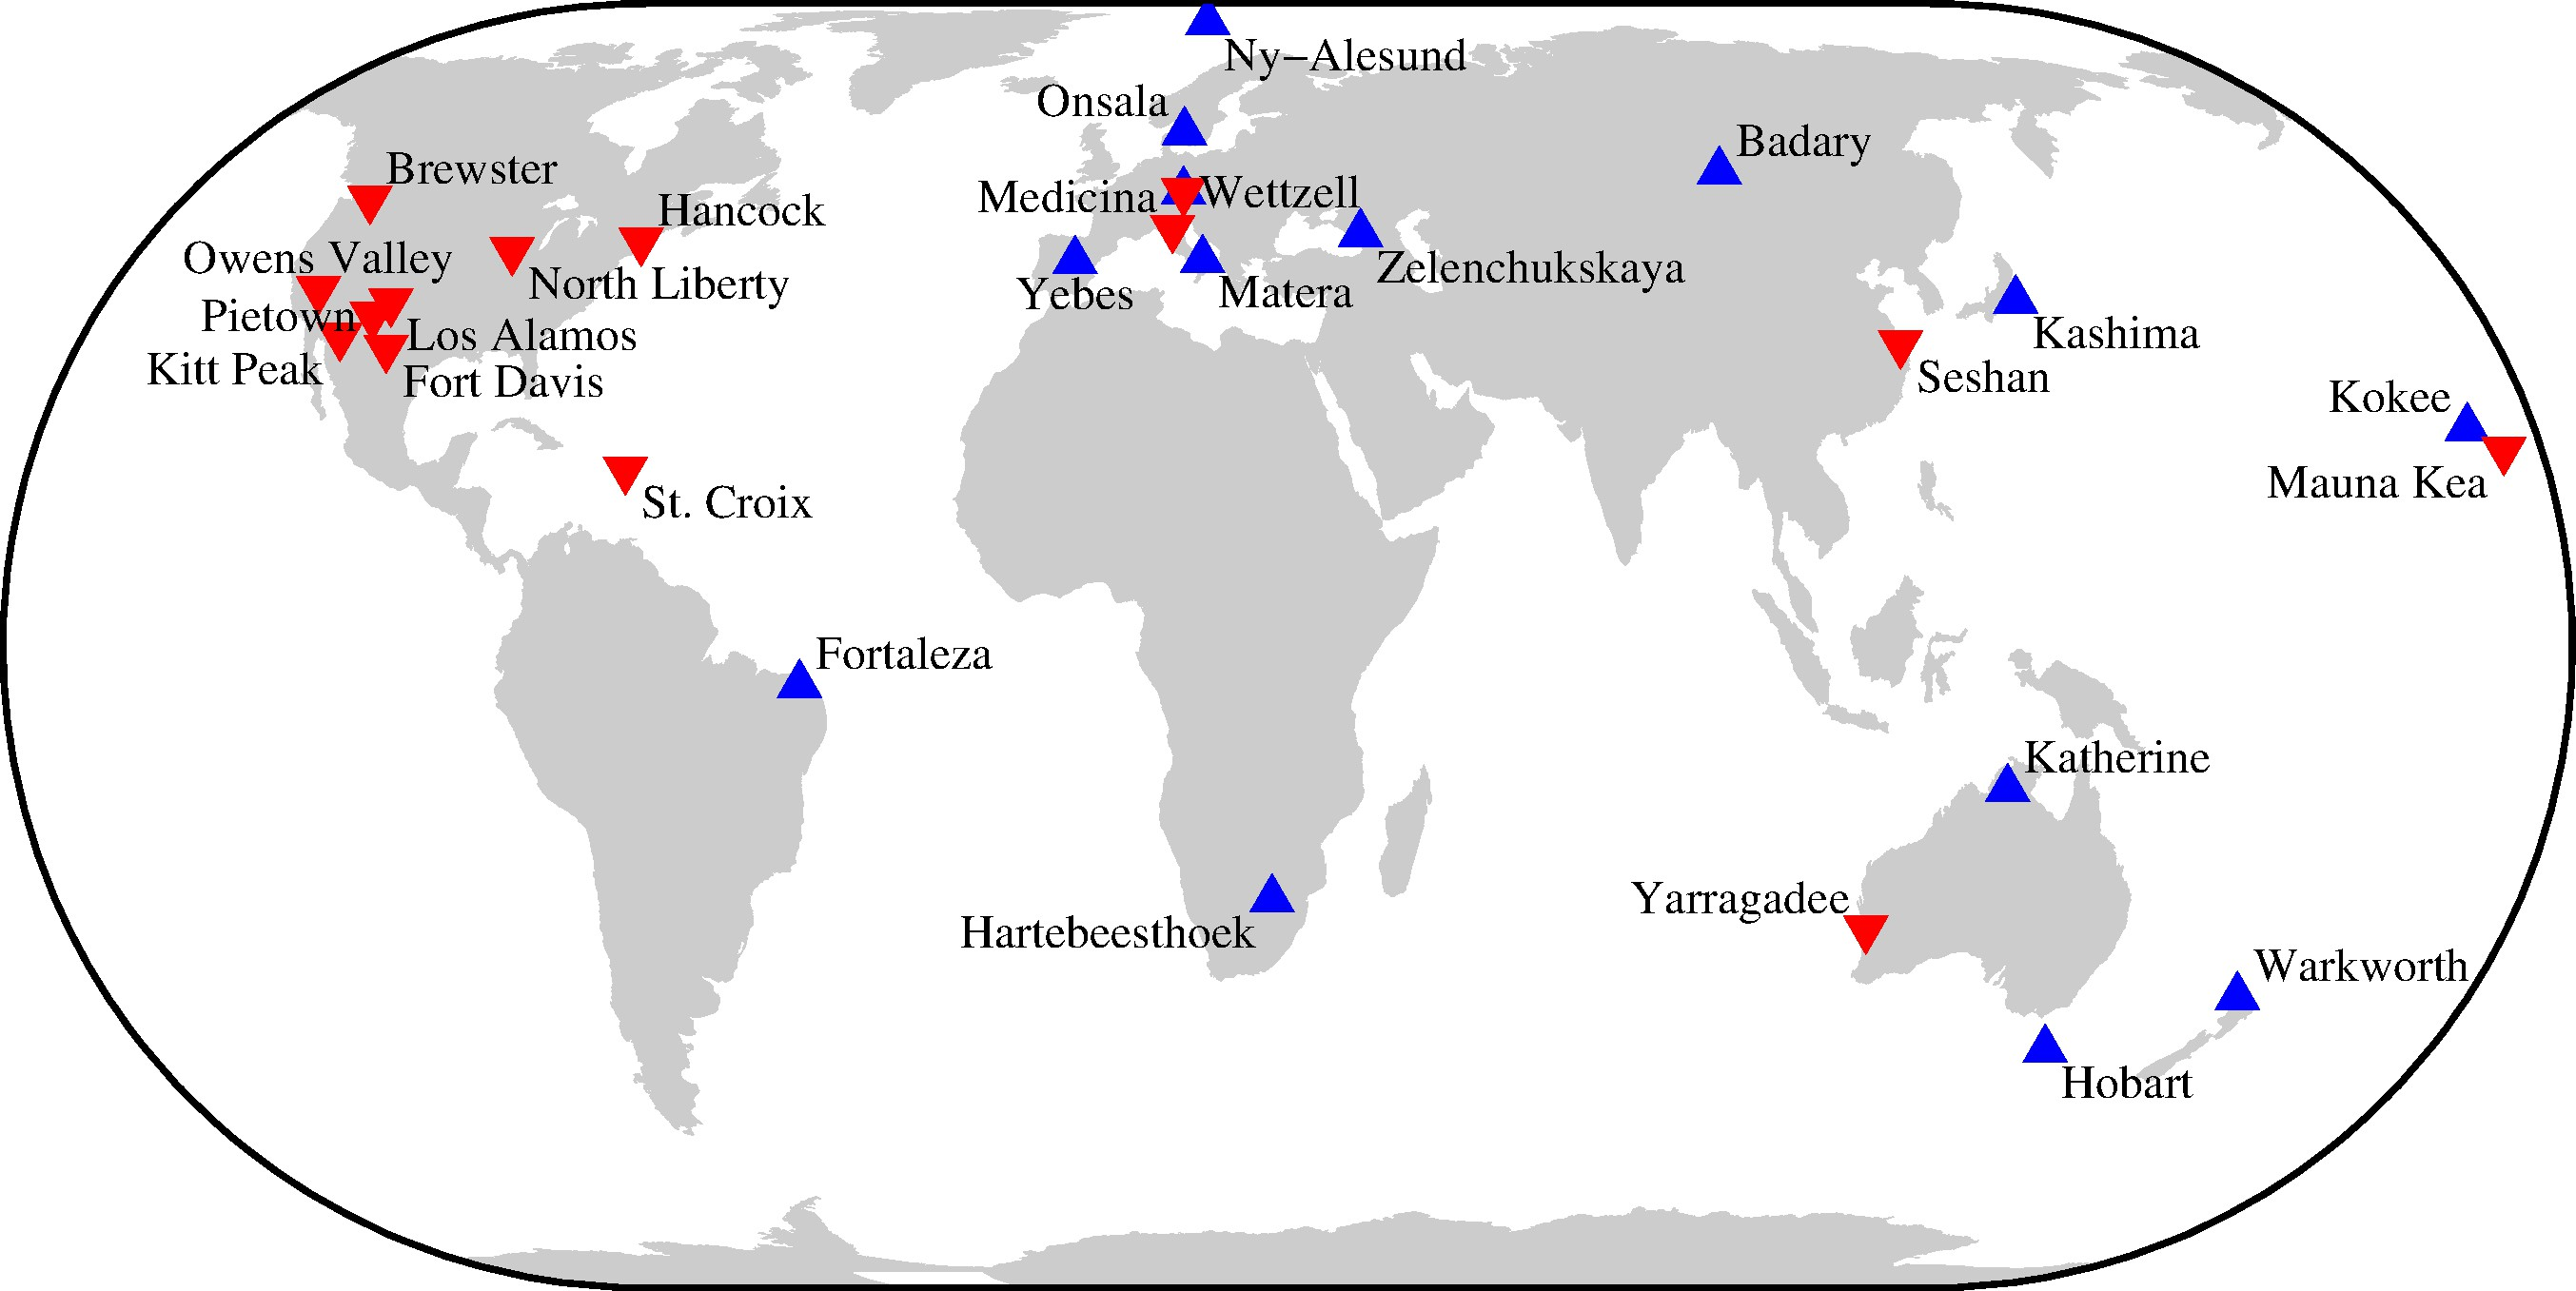
\includegraphics[width=0.6\columnwidth]{cont17_legacy.jpg}
	\caption{Radio telescopes used for CONT17. Both blue and red markers
	indicate legacy stations used for measurements in past sessions.}
	\label{fig:vlbi_locs}
\end{figure*}


Determining the rotation of the Earth allows us to understand the vast phenomena that occur on Earth,
including tidal breaking, seasonal variations, and the Chandler wobble, the nutation that occurs with Earth's
rotation axis. Furthermore, climate change has a strong effect on the rotation rate as the melted ice from the 
polar ice caps gravitate towards the equator, increasing the angular momentum and thus the rotation period of Earth.
This is shown to increase at a rate of $\SI{1.2}{\micro\second}$ per year \cite{Groh2021}. \par 

While the VLBI can determine the rotation rate with high precision, due to the operation times the temporal resolution
is low. As such, transient events such as earthquakes and tides cannot be resolved. As of such, 
laser gyroscopes have been employed to resolve such details. While it lacks in the long-term stability of VLBI,
they have a temporal resolution of approximately an hour or less \cite{Wettzell2005}. The G-ring at the German
Fundamentalstation Wettzell is one of the best ring laser gyroscopes with a sensitivity of around \SI{12}{\pico\radian\per\second\per\sqrt{\hertz}} \cite{Groh2021}. 
See Fig. \ref{fig:gring_gyro} for an image and the setup of the G-Ring gyroscope. Ring laser gyroscopes are still explored today to 
describe other phenomena from the Earth's rotation such as the Lense-Thirring Effect, and gyroscopes such as the GINGERino have been proposed to 
measured such quantities \cite{Beverini2016}.

\begin{figure*}[h!]
	\centering
	\subfloat[]{{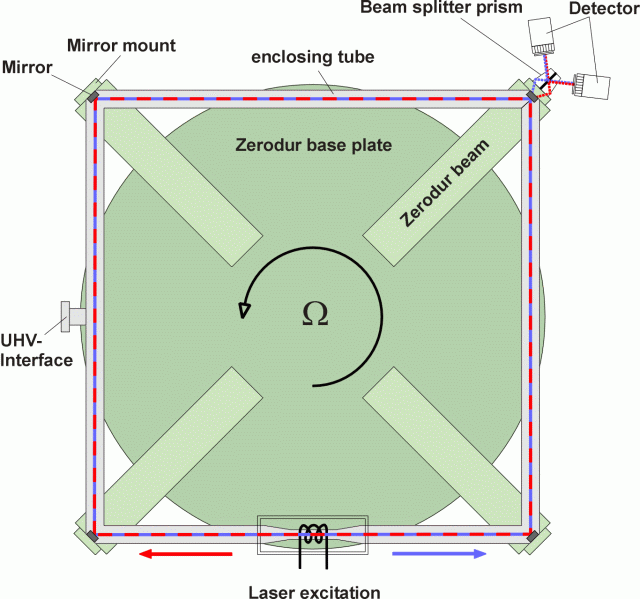
\includegraphics[width=0.4\columnwidth]{gring_gyroscope.png}}}
	\quad
	\centering
	\subfloat[]{{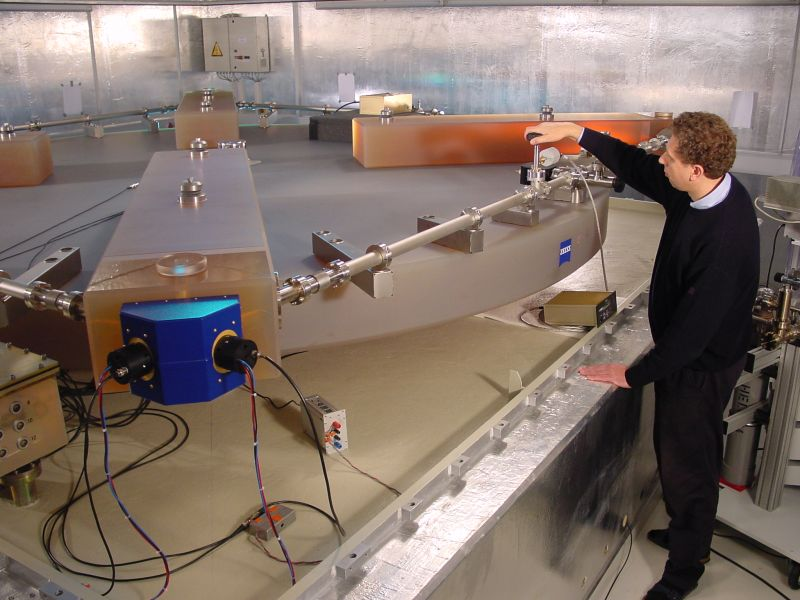
\includegraphics[width=0.4\columnwidth]{G-ring.jpg}}}
	\caption{The G-Ring gyroscope at the Fundamentalstation Wettzell. (a):
	The setup of the gyroscope. (b): Image of the G-ring. Obtained from Ref. \cite{Wettzell2005}.}
	\label{fig:gring_gyro}
\end{figure*}

% The first time that a ring laser gyroscope was employed for measurement of the rotation of the Earth was 
% from the Michelson-Gale experiment, conducted in 1929. In such experiment, Albert A. Michelson sent counter-propagating beams thorough 
% pipelines with a total effective area of around $\SI{0.2}{\kilo\metre\squared}$. He observed that the fringe difference measured
% was well within the expectations of the analytical fringe shift \cite{Groh2021}. 

% add something about the Michelson-Gale experiment here? maybe not needed. otherwise can also add another figure too

In our experiment, we use a ring laser gyroscope to attempt to measure the rotation rate of the Earth. This is done by employing the Sagnac effect,
which allows us to determine the rotation of an inertial system by the path length difference between two light beams. To observe
the quality of the constructed laser gyroscope, we measure optical cavity parameters such as the free spectral range,
PDH locking error signals, lock-in threshold, and the finesse. We further quantify the stability and sensitivity of the gyroscope by 
determining the Allan deviation. \par 

This paper is structured as follows. Chapter 1 motivates the experiment by elaborating on the usage of ring laser gyroscopes
to determine the rotation rate of the Earth. Chapter 2 describes the theory behind the quantities measured in the experiment. Chapter 3
describes the setup used in our experiment and the method used to determine the relevant quantities for each part of our experiment. 
Chapter 4 shows the pre-laboratory tasks that were required before starting the experiment. Chapter 5 shows the results
that we have obtained and discussions related to the results. Finally, we summarize our findings and address possible outlooks for our experiment
in Chapter 6. 

% should we hyperlink the chapters?


\chapter{Theory}

\section{Gyroscopes}

\subsection{The Sagnac Effect}

The Sagnac effect tells us that whilst the motion between two inertial frames cannot be distinguished, two rotating frames can be 
distinguished, allowing one to directly measure the rotation rate of an inertial system \cite{Groh2021}. This effect was first observed by 
George Sagnac in 1913, whom believed that this experiment was a proof that aether exists in an inertial frame  \cite{Darrigol2014}. This, however, was 
disproven by Max von Laue in 1911 where he showed that the Sagnac effect was compatible with special relativity \cite{Laue1911}. 
However, the interpretation of the Sagnac effect due to the general theory of relativity is still investigated today, 
even though it is already well-known in literature \cite{Benedetto2019}. In our analysis, we utilize the Sagnac effect on a gyroscope to 
measure the rotation rate of the Earth.\par

To observe the Sagnac effect, we consider an interferometer setup with light propagating with wavelength $\lambda$ enclosing an area $\vec{A}$
 with perimeter $P$. Placing such a setup onto a rotating platform with frequency $\vec{\Omega}$, we observe that the optical path that
 each light travels changes. For example, if the table rotates counter-clockwise, then the path of the co-rotating light increases, while that of the other light
decreases (see Fig. \ref{fig:sagnac_effect}). The Sagnac effect then tells us the resulting phase shift between the two lights:
\begin{equation}
	\delta \phi = \frac{8\pi \vec{A} \cdot \vec{\Omega}}{c \lambda} \propto \vec{A} \cdot \vec{\Omega}
\end{equation} 

\begin{figure*}[h!]
	\centering
	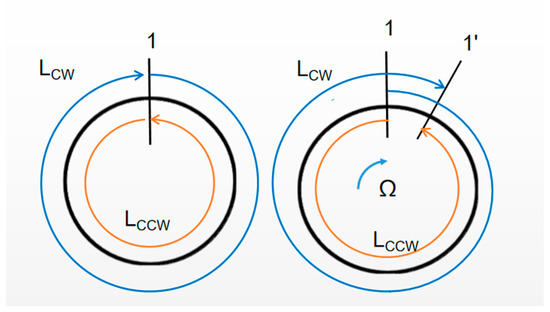
\includegraphics[width=0.6\columnwidth]{sagnac_effect.jpg}
	\caption{The Sagnac effect. \textit{Left}: Setup without rotation. The beam moving clockwise (blue) and counter-clockwise (orange)
	have the same optical path length. \textit{Right}: Setup with a clockwise rotation $\Omega$. The path length of the 
	clockwise beam is larger than that of the counter-clockwise beam. Obtained from Ref. \cite{Feng2020}.}
	\label{fig:sagnac_effect}
\end{figure*}

A more detailed derivation using the relativistic law of velocity addition can be found in Ref. \cite{Benedetto2019}. 

\subsection{Ring Laser Gyroscopes}

\subsubsection{Active Ring Laser Gyroscopes}

In order to incorporate the Sagnac effect within our experiment, we utilize ring laser gyroscopes. A laser is placed within an 
enclosed cavity, and emits two counter-propagating beams. Such beams reflect off mirrors and interfere at the end of their 
propagation. When rotating the platform in which such setup is placed, different interference patterns can be observed, and 
transforms the ring cavity system into a cavity resonator. The corresponding beat frequency $\delta \nu$ observed is then the 
Sagnac frequency, which is given as such:

\begin{equation}
	\delta \nu = \frac{4 \vec{A} \cdot \vec{\Omega}}{P \lambda}
	\label{eq:sagnac_freq}
\end{equation}

In our experiment, we only consider square ring cavities so that $A = L^2$ and $P = 4L$, where $L$ is the path length of each arm. 
As such, we can simplify Eq. \ref{eq:sagnac_freq} as such: 
\begin{equation}
	\delta \nu  = \frac{L \Omega}{\lambda} = n \Omega
\end{equation}
where $n = L / \lambda$ is the number of nodes of the light field in each arm. Thus the Sagnac frequency is proportional to the rotation rate
of the inertial system \cite{Groh2021}.\par 

\subsubsection{Passive Ring Laser Gyroscopes}

In contrast to the active ring laser gyroscope, in which the laser is contained within the ring cavity, the passive ring laser
gyroscope places the laser source outside of the cavity system. In this system, the external laser is locked to the counter-propagating
modes of the resonator. By placing the laser outside of the resonator, we can reduce the systematic effects due to the lasing medium and 
the lock-in effect (see Sec. \ref{sec:lockin_effect}), and also increase the available light power for the beam. 
This method, however, also introduces an added complexity of laser locking \cite{Groh2021}. See Fig. \ref{fig:passive_active} for a comparison between the two
systems. In our experiment, we use the passive ring laser gyroscope and thus laser locking becomes an importance in our measurements.

\begin{figure*}[h!]
	\centering
	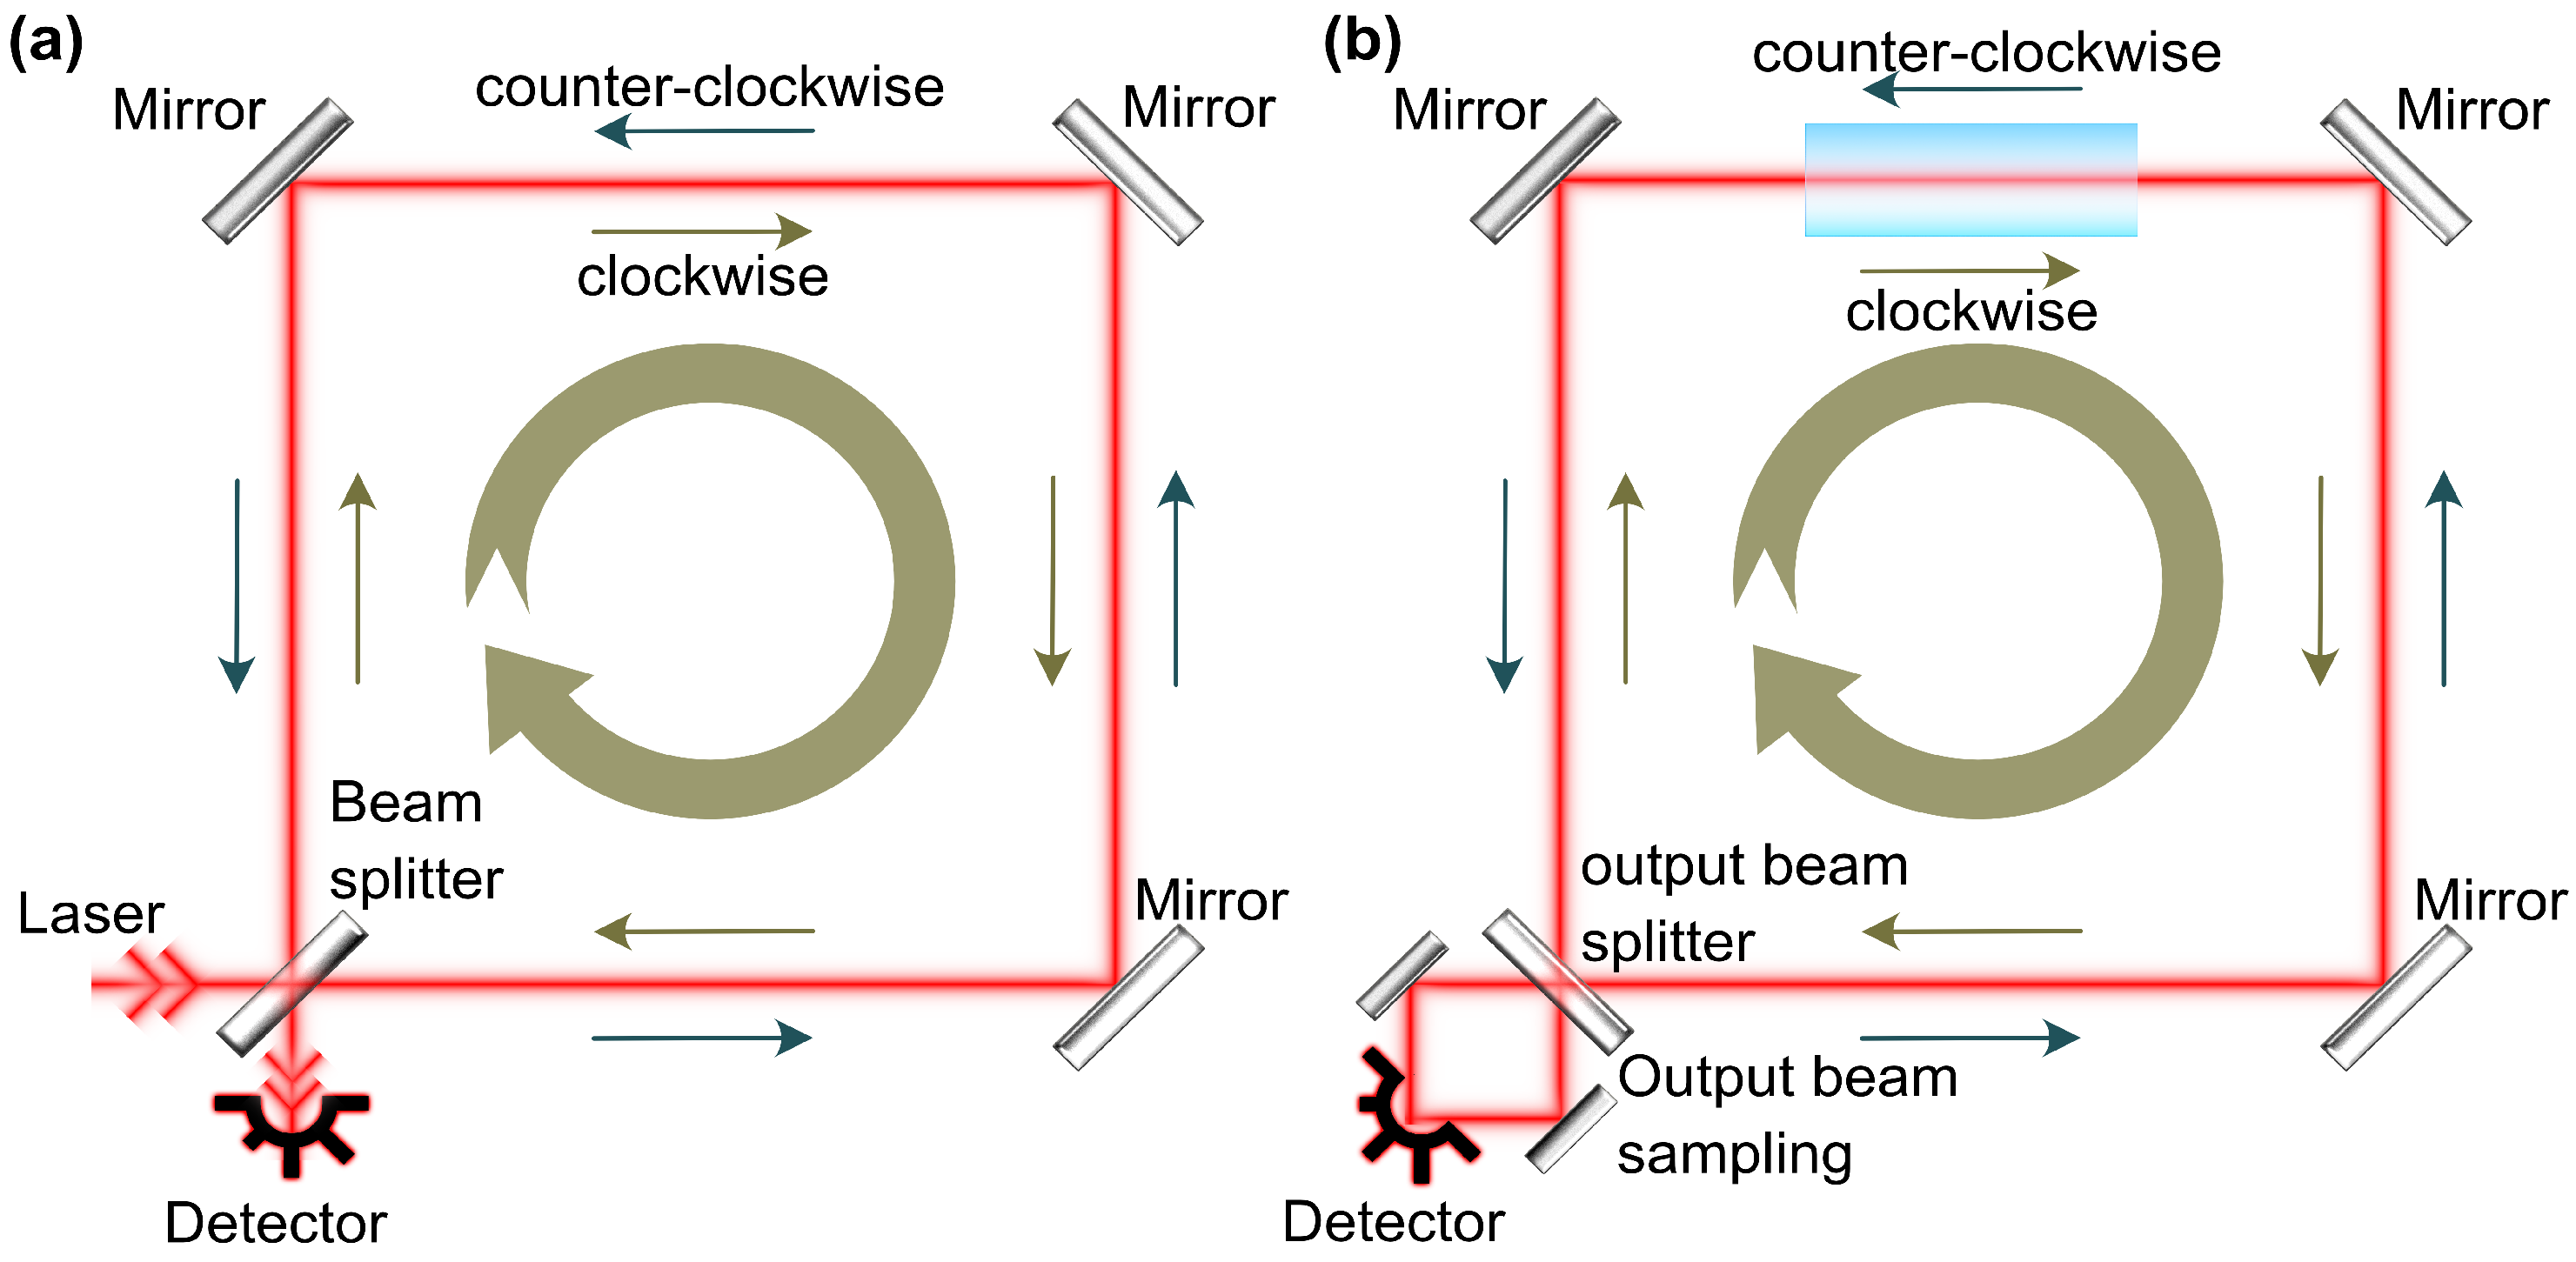
\includegraphics[width=0.6\columnwidth]{passive_active_gyroscope.png}
	\caption{Ring laser gyroscope systems. \textit{Left}: Passive, \textit{Right}: Active. Obtained from Ref. \cite{Kudelin2021}.}
	\label{fig:passive_active}
\end{figure*}

\subsubsection{Gyroscope Sensitivity}

The sensitivity of the ring laser gyroscope depends on a variety of factors, namely the wavelength $\lambda$, arm length $L$, finesse $F$
of the resonator (see Sec. \ref{sec:finesse}), and the shot-noise limited detection given by the number of photons $N = P_{\text{opt}} / h \nu = P_{\text{opt}} \lambda / hc$ detected per unit time. 
$P_{\text{opt}}$ represents the optical power given to the laser. Combining all such factors, we obtain the sensitivity of the ring laser gyroscope for an integration time $\tau$ as such: 
\begin{equation}
	\delta \Omega = \frac{1}{4} \frac{c}{L^2F}\sqrt{\frac{ch\lambda}{P_{\text{opt}}}} \frac{1}{\sqrt{\tau}}
	\label{eq:gyroscope_sensitivity}
\end{equation}

This gyroscope sensitivity can be directly compared with the Allan deviation $\sigma_{\text{ad}}$ that determines the instability of 
a measurement for some averaged integration time $\tau$ (see Sec. \ref{sec:allan_dev}). 

\section{Optical Cavities}

A cavity is a hollow conductor which contains electromagnetic waves going in and reflecting off the walls. At certain frequencies, these reflected waves form standing waves which correspond to the resonant modes of the cavity. An optical cavity consists of an arrangement of mirrors, which produces standing electromagnetic waves. In our setup, instead of the traditional Fabry-P\'erot interferometer, which consists of two opposing flat mirrors, we use four mirrors. Nevertheless, the same principles of resonance modes applies.

\subsection{Cavity Modes}

The solution to optical resonators with parabolic mirrors and homogeneous medium is given by the Hermite-Gaussian modes. The Hermite-Gaussian modes are the solution to the paraxial Helmholtz equation, when considering Cartesian coordinates with the beam propagating along the $z$-axis. 



% include this somewhere
\begin{equation}
	\delta\nu_{\text{FSR}} = \frac{c}{P}
	\label{eq:fsr}
\end{equation}

\subsection{Finesse} \label{sec:finesse}

\subsection{Lock-In Effect} \label{sec:lockin_effect}


\section{Allan Deviation} \label{sec:allan_dev}

The Allan deviation is used to quantify the instability of any device that measures differences in frequencies. Assuming that the
measurement is only limited by the photon shot-noise (amongst others), we can describe the Allan variance as the deviation
between temporal averages of measurements $y$ over some time interval or integration time $\tau$:
\begin{equation}
	\sigma_{{\text{ad}}}^2 = \frac{1}{2M} \sum\limits_{n=1}^M (\bar{y}(\tau)_{n+1} - \bar{y}(\tau)_n)^2
\end{equation}
where $M$ is the number of samples. The Allan deviation is then the square root of the variance. \par 

The Allan deviation is especially helpful to understand the sensitivity in gyroscopes. Imposing the same assumptions as above,
we can describe the Allan deviation with typical shot noise scaling $\propto 1 / \sqrt{\tau}$ as such:
\begin{equation}
	\sigma_{\text{ad}} = \frac{\mathcal{A}}{\sqrt{\tau}}
\end{equation}
where $\mathcal{A}$ (given in $\si{\radian\per\second\per\sqrt{\hertz}}$) is known as the sensitivity of the gyroscope. This 
value can be directly compared with the theoretical gyroscope sensitivity (per integration time)
described in Eq. \ref{eq:gyroscope_sensitivity} \cite{Groh2021}.



\chapter{Pre-Lab Exercises}

Before conducting the experiment, we were required to determine the rotation rate of the Earth using our phone. Our phones
contain a microelectromechanical system (MEMS), which is a portable and inexpensive inertial sensor that track the motion of
the phone. Using the application \texttt{phyphox} constructed by RWTH Aachen University, we evaluated the capabilities
of the MEMS gyroscope within our phones. 

\section{Task 1: Getting Started}



\section{Task 2: Allan Deviation} \label{sec:prelab_allan_dev}

\section{Task 3: Rotation Rate of Earth}



\chapter{Experimental Set-Up and Procedure}

\section{Experimental Set-Up}

% Here we should describe how we set-up the laser gyroscope until it works for our measurements
% so we should mention the following in the procedure section (NOT in this section, to avoid overlap):
% - measuring free spectral range
% - measuring error signal
% - measuring other things like 

\section{Procedure}

\subsection{Free Spectral Range}

We first measured both the signal of the laser input and after the laser
has passed through the ring cavity system. The window was adjusted until three resonance peaks and their corresponding sidebands
were observed. See Fig. \ref{fig:threeres_raw} the observed raw signal. 

\begin{figure*}[h!]
	\centering
	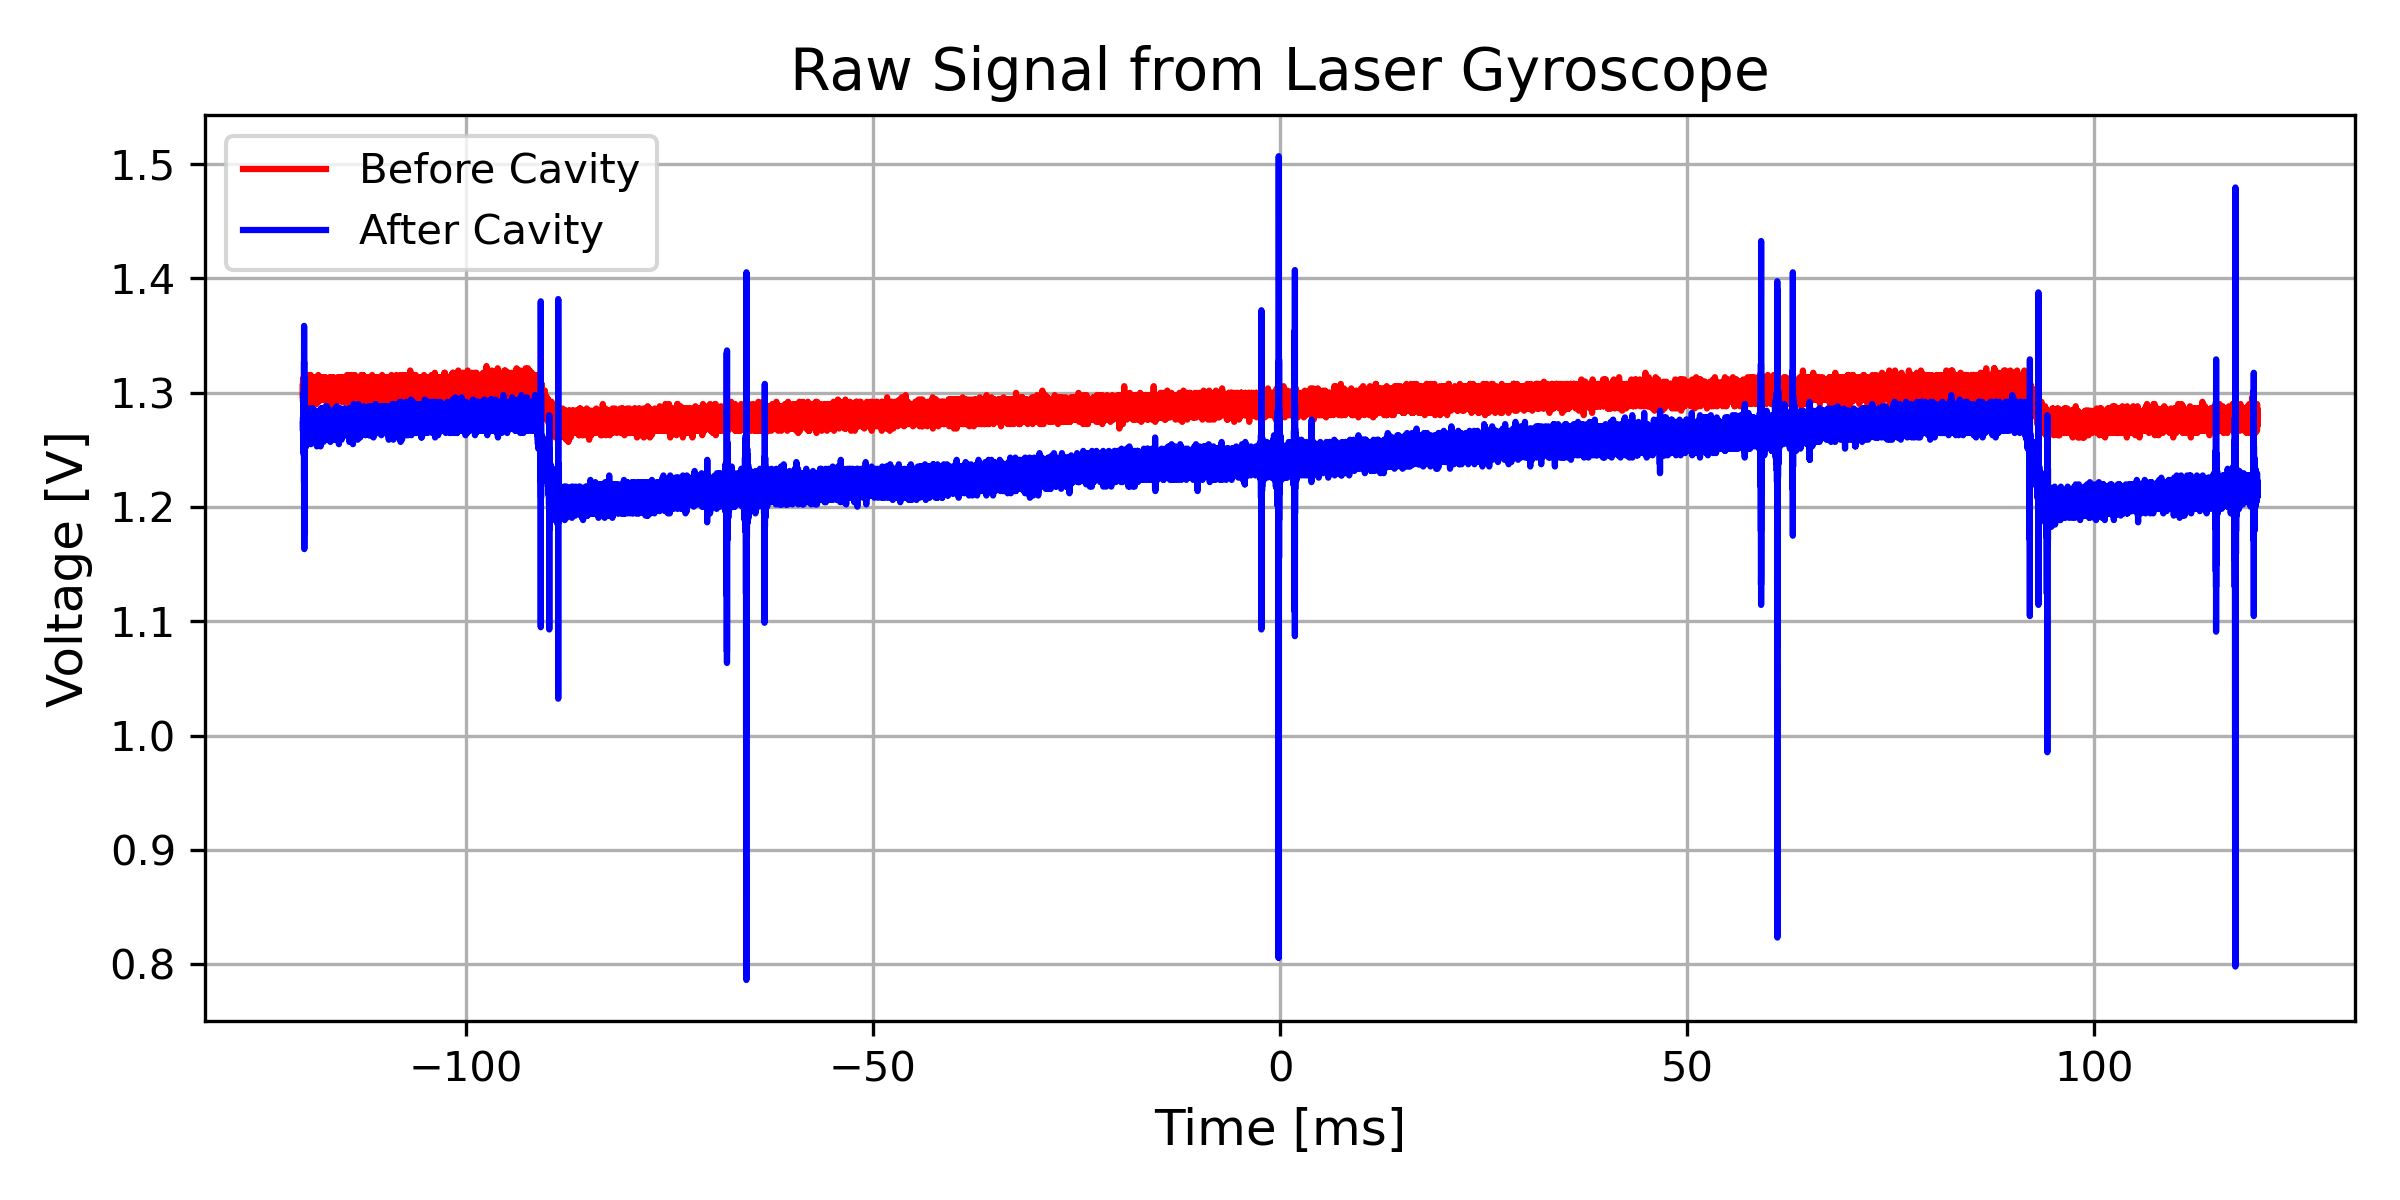
\includegraphics[width=0.8\columnwidth]{threeres_raw.png}
	\caption{Raw signal input from the laser before and after passing through the ring 
			cavity system.}
	\label{fig:threeres_raw}
\end{figure*}

As the raw data was provided in the time domain, we converted the time axis into a frequency axis.
In order to do so, we use the fact that the modulation frequency from the EOM was $\Omega = \SI{10}{\mega\hertz}$,
and we determined the width in time between the peaks and the sidebands to obtain a conversion factor between 
the two axes. From this conversion factor, we obtained the free spectral range as the peak-to-peak difference between
the resonance peaks. We also took the average of the values to obtain a mean free spectral range.

We then evaluated the cavity perimeter from Eq. \ref{eq:fsr} for each free spectral range that we have observed.
We compared our obtained results with the measured value of the cavity perimeter
 $P_{\text{meas}} = \SI{0.990\pm 0.005}{\meter}$ obtained from Ref. \cite{Groh2021}. 


\subsection{PDH Error Signal}

To observe the error signal generated from PDH locking, we observed the combined signal generated from the fast and slow PID controller. Fig. \ref{fig:errsig_raw} shows the raw signal obtained from the PDH error.  The corresponding data was then used to determine the linear fit of the error signal where the zero crossing and 
linear slope is present (i.e. near the middle of the observed error signal). The linear fit was obtained by using \texttt{numpy.polyfit}. \par 

\begin{figure*}[h!]
	\centering
	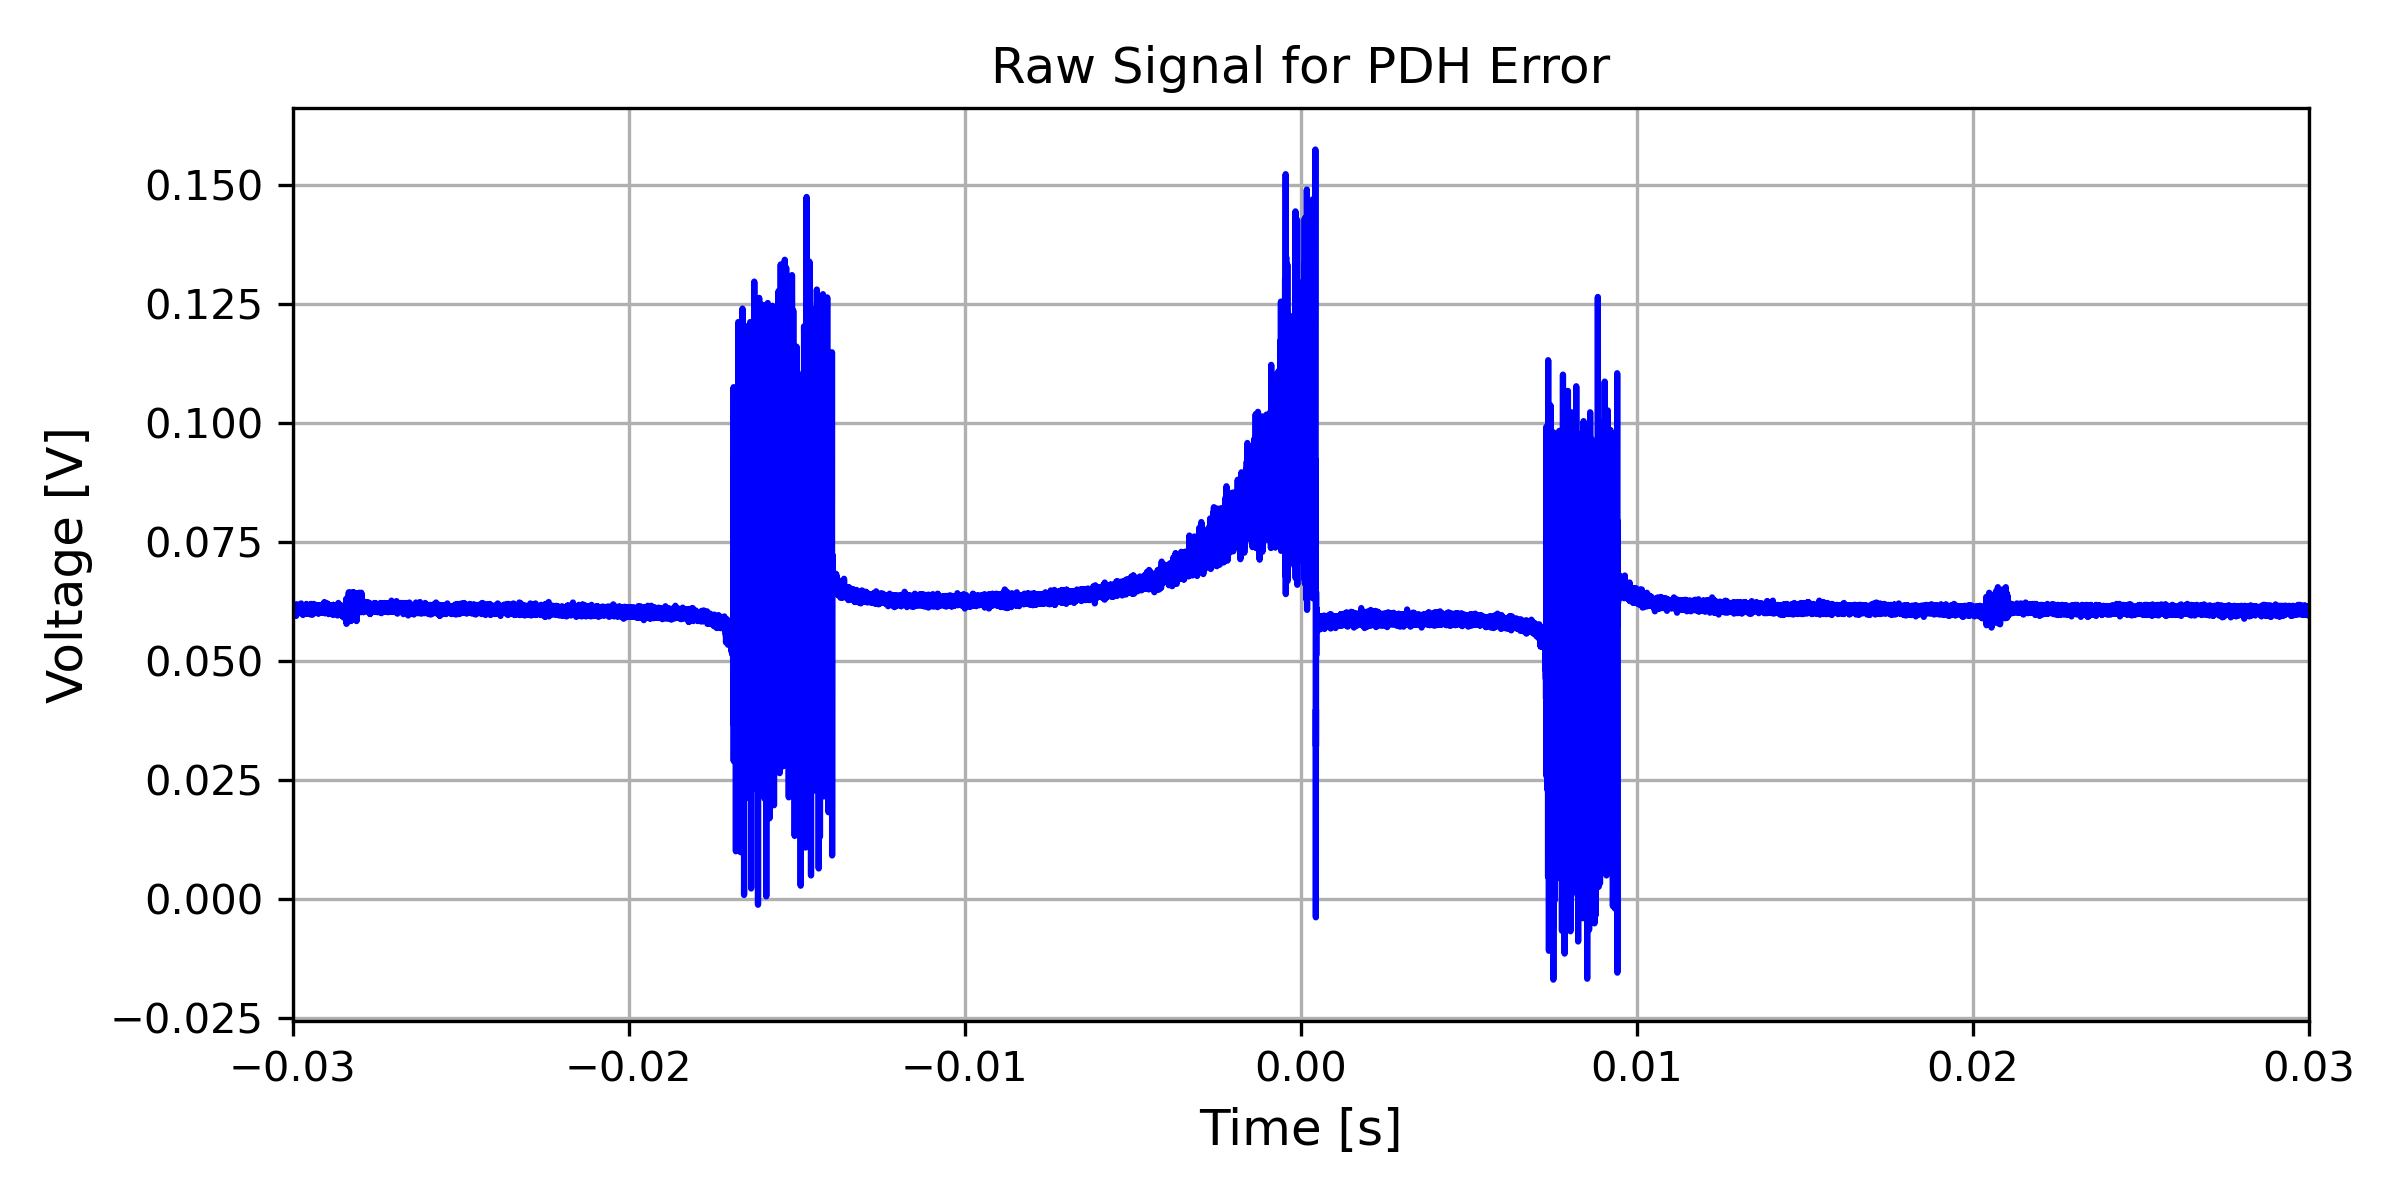
\includegraphics[width=0.8\columnwidth]{raw_err_sig.png}
	\caption{Raw Signal from PDH locking using the fast and slow PID controller.}
	\label{fig:errsig_raw}
\end{figure*}


The error signal was then used to determine the optimal PID parameters that yield the most stable and large signal. In order to 
do this, the following parameters were modified: SLOW INT, FAST INT, DIFF GAIN, FAST DIFF / FILTER, SLOW GAIN, FAST GAIN, GAIN LIMIT, and OFFSET. The major parameters that influenced the signal were the SLOW INT, SLOW GAIN, FAST DIFF / FILTER and FAST GAIN. Modifying the SLOW INT and FAST DIFF caused the laser to be out of lock, whereas FAST GAIN decreased the noise observed in the signal. As we decreased the SLOW GAIN, we observed that the laser became more out of lock, allowing for the control of the laser locking. The OFFSET parameter adjusted the offset between the two signals. Table \ref{tab:pid_params} shows the optimal PID parameters used in the subsequent measurements which were both stable and yielded a strong signal strength. \par 

\begin{table}[h!]
	\centering
	\begin{tabular}{|c|c|}
		\hline 
		PID Parameter & Value \\ \hline
		SLOW INT & 25 \\ \hline
		FAST INT & 20K \\ \hline
		FAST DIFF / FILTER & 10M \\ \hline
		FAST GAIN & $\SI{6}{\decibel}$ \\ \hline
		GAIN LIMIT & 30 \\ \hline
	\end{tabular}
	\caption{The optimal PID parameters used for this experiment. The SLOW GAIN and FAST GAIN parameter values are not noted
	as specific values are not marked on the Moglabs PID controller.}
	\label{tab:pid_params}
\end{table}

When performing laser locking, we further needed to consider the systematics due to the environment. Any small disturbance such as clapping, tapping the desk, moving the cables or even walking influenced the degree of locking for the laser. Other factors such as the temperature fluctuations in the room may have caused the laser to be out of lock as well. \par 


\subsection{Cavity Ring-Down}

\subsection{Scale Factor} \label{sec:scale_fact}

\subsection{Allan Deviation}

Finally, we measured the Allan deviation of the laser gyroscope. We performed the same procedure as with the scale factor measurement. 
Using the same PID parameters as before, we set the rotation frequency to rotate with $\SI{0.75}{\volt}$, so that the laser will 
remain locked as long as possible. The gyroscope was rotated until the cable connecting the gyroscope did not extend or contract
any further, then the same analysis was performed in the opposite rotation direction. The measurement was taken continuously for 
approximately 1.5 hours. The unprocessed time series for the frequency measurement can be seen in Fig. \ref{fig:allan_ts_raw}. \par 


\begin{figure*}[h!]
	\centering
	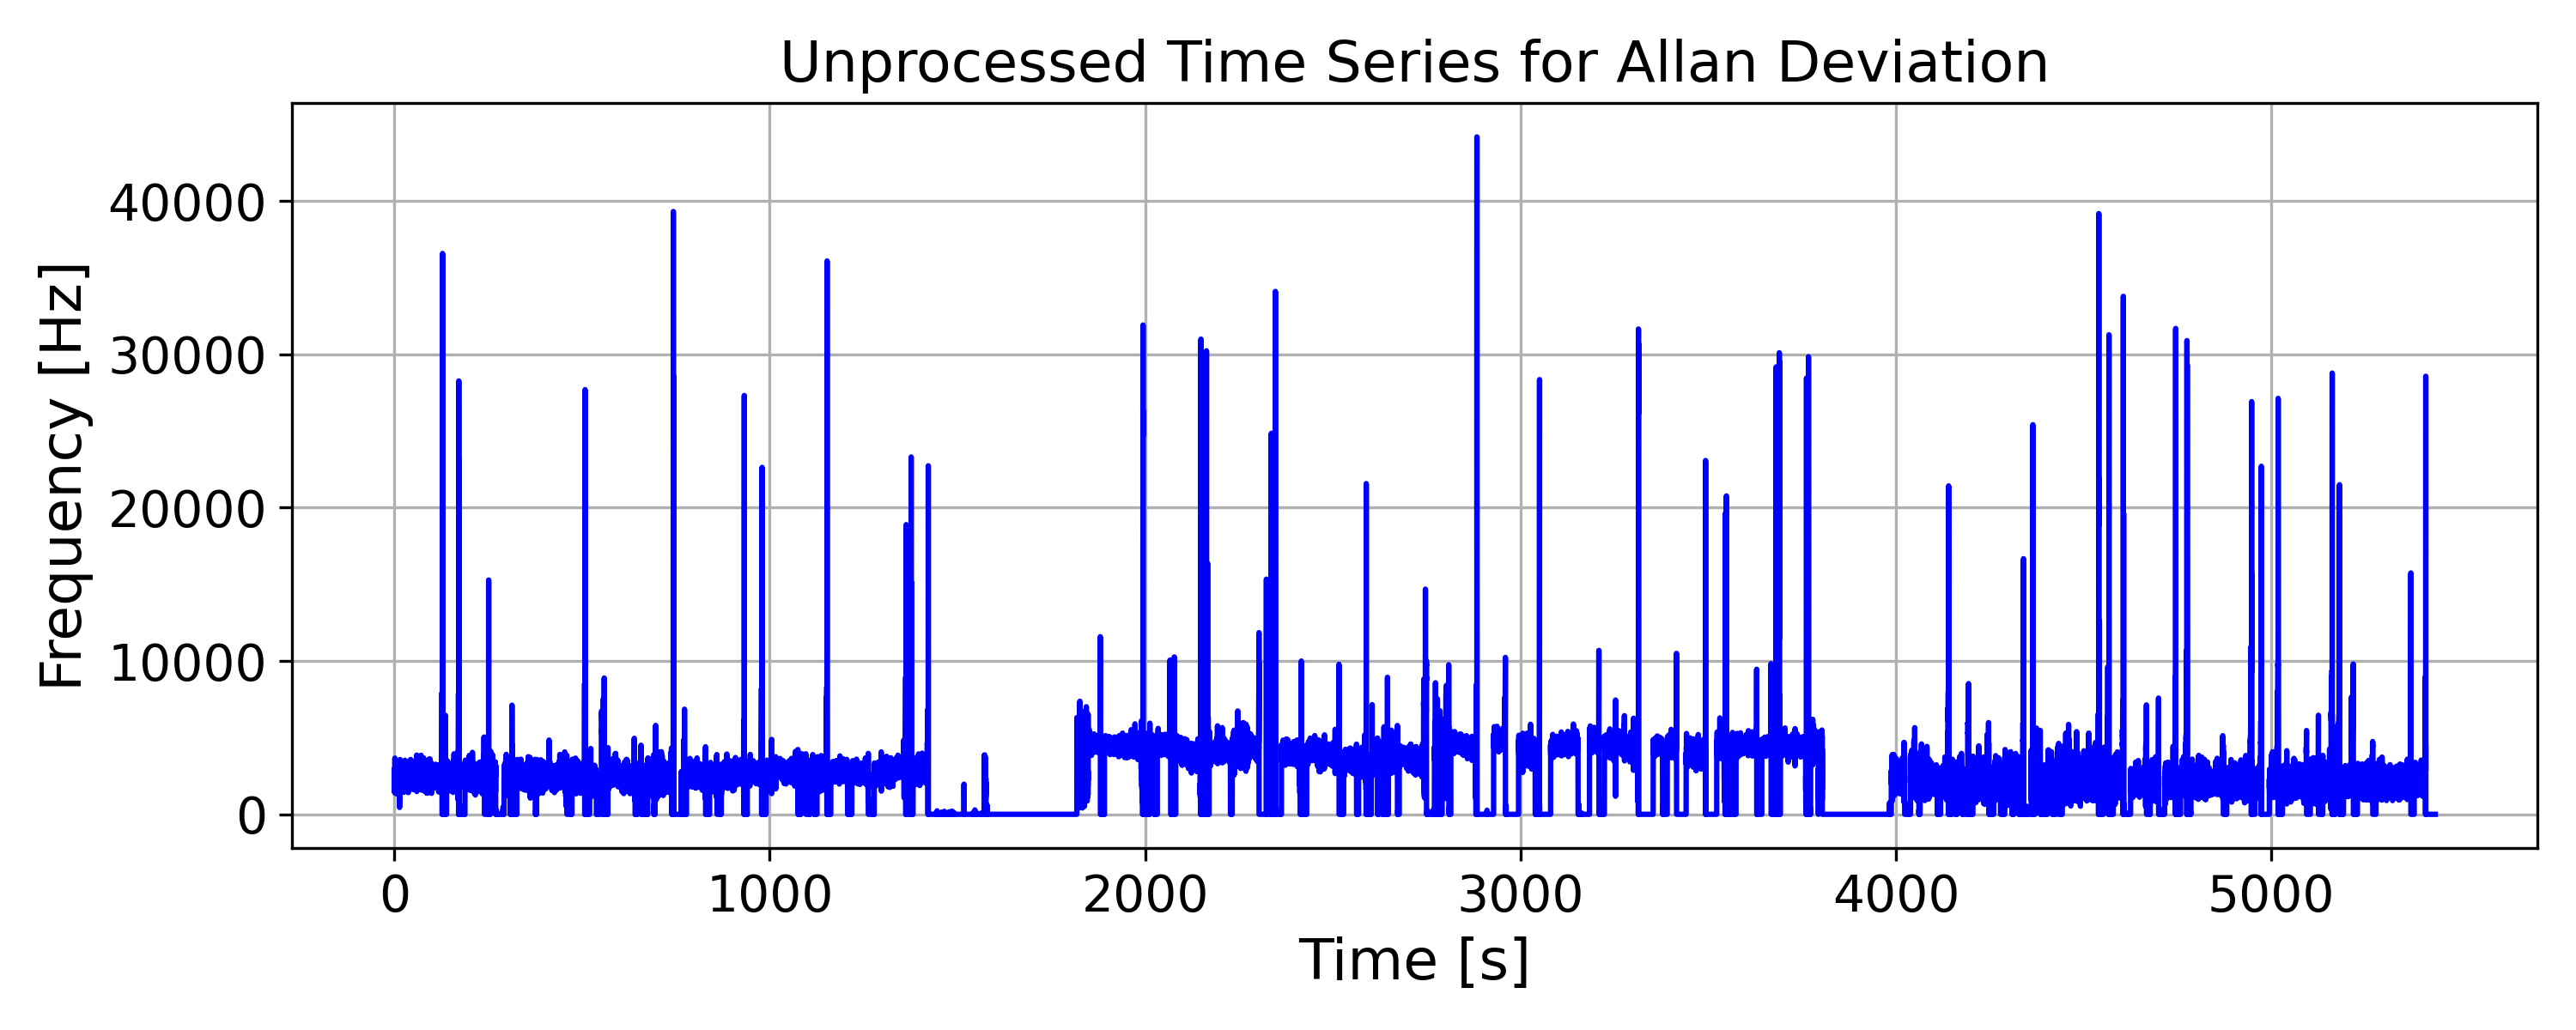
\includegraphics[width=0.8\columnwidth]{allan_ts_raw.png}
	\caption{Unprocessed time series obtained from Allan deviation measurements. We observe large
			spikes at numerous locations as well as regions with zero frequency.}
	\label{fig:allan_ts_raw}
\end{figure*}

From the raw data, we first removed any measurements that were taken while the laser was unlocked and when the 
rotation of the table was switched. After applying some filtering to the data (using \texttt{scipy.signal.sosfilt}), we then performed
the same procedure as with the Pre-lab tasks in Sec. \ref{sec:prelab_allan_dev} to determine the Allan deviation.
We also determined the shot-noise limited time $\tau$ by observing the time duration in which the instability of the 
measurement starts. For the rotation frequency of the table, we followed the same procedure from Sec. \ref{sec:scale_fact}. \par 

% $\Omega = \SI{5.95\pm 0.75}{\hertz}$


\chapter{Results and Discussion}

\chapter{Conclusion and Outlook}

\chapter{Acknowledgements}

\printbibliography

\chapter{Appendix}

\printbibliography

\end{document}
